\subsection{\rqthree}
\label{sec:results:rq3}
\subsubsection{Motivation}
In the previous research question, we looked at how clients respond to in-range breaking updates. However, while it is the client's build that is failing, the root cause of the issue could originate from the provider. In this research question, we look to see whether in-range breaking updates prompt a response from the provider packages.
\subsubsection{Approach}
Initially, we examined all of the comments made by users on the in-range breaking build issue reports looking for potential references to issue report made in the dependency package that were related to the client's breaking build issue report. We were not successful in finding any, so we took a different approach. We hypothesis that, if a release from a package provider causes an in-range breaking builds in a high proportion of client, the next release the provider package makes would happen quicker than usual. To test this, we compare the average release frequency of packages against the time it takes a package to release the next update immediately following an update that causes an in-range breaking build in at least 20\% of clients that depend on it.
\par
First, we determine the number of clients that are using each of the provider packages we have release information on in our data set. We then determine how many issue reports were opened for each release made by each provider package. Using this information, we determine the ratio of in-range breaking update issue reports that each release made by every provider package caused. This allows us to categorize each release either as a breaking release or a non-breaking release. We then compare the release frequency of the non-breaking releases to the time to the release immediately following each breaking release.

\subsubsection{Results}
We first used all release records in our analysis including releases that did not cause any in-range update breaking issues in any clients. We found that the median release time after non-breaking releases was 1 day and 22 hours (IQR = 3 hours - 10 days 12 hours), while the median release time immediately following a breaking release was 8 days and 6 hours (IQR = 1 day and 3 hours - 39 days and 6 hours). From these results, it appears that the release that immediately follow an update that breaks a proportion of clients tends to take longer to be made available. However, we choose to perform further analysis on only breaking releases.
\par
We examine only the set of releases that caused at least one in-range breaking build issue report to be opened in a client. While all these releases caused at least one breaking build, we still classify a breaking release as a release that caused at least 20\% of the package's client's builds to break. The median release time immediately following a breaking release was still 8 days and 6 hours (IQR = 1 day and 3 hours - 39 days and 6 hours), as that data set was unaffected, but the median release time after non-breaking releases was 8 days and 6 hours (IQR = 1 day 3 hours - 39 days 6 hours). These results can be seen in Figure \ref{fig:time_until_next_breaking_release}.
\begin{figure*}[h]
    \centering
    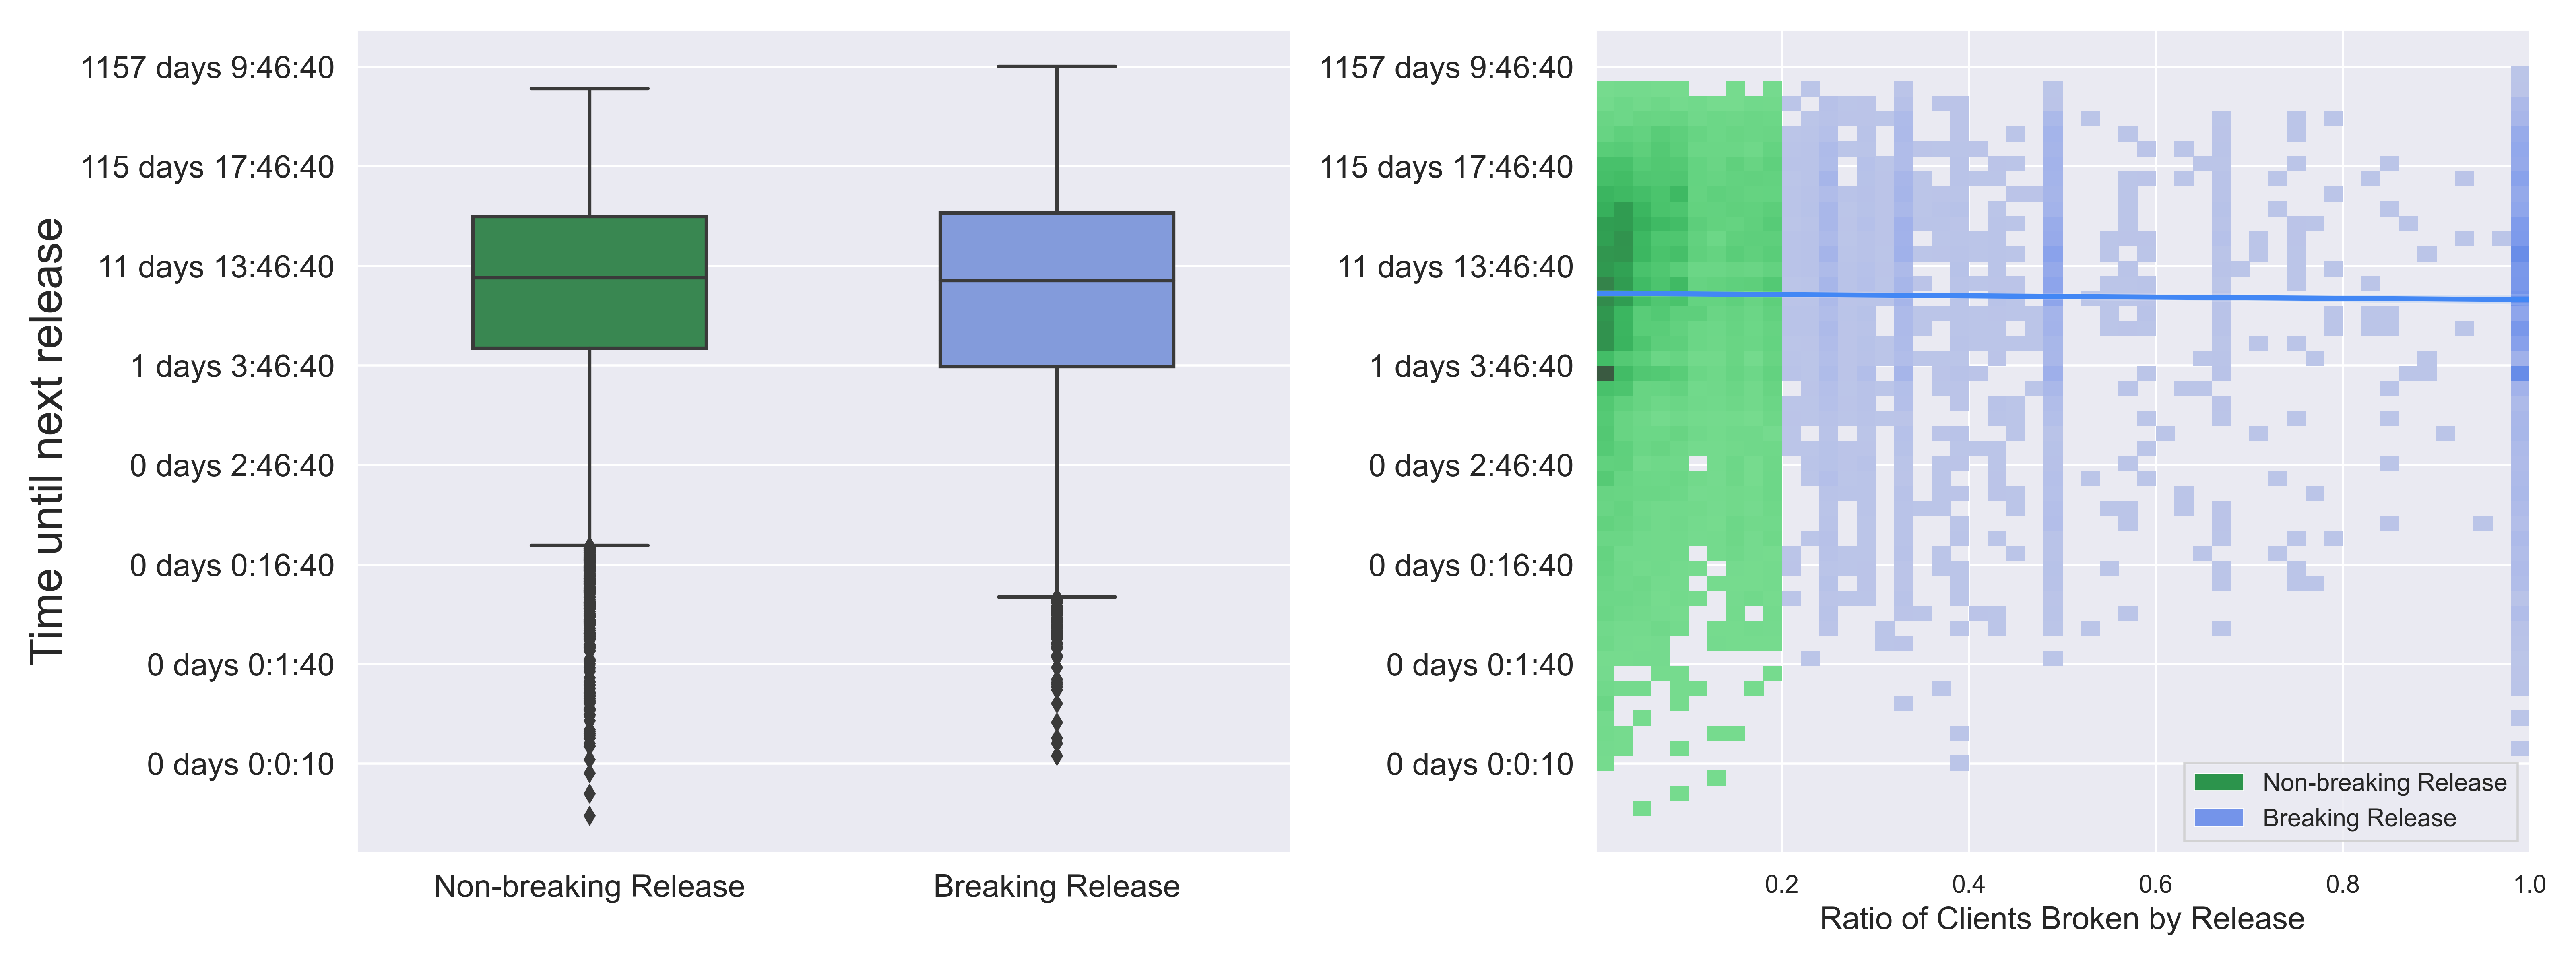
\includegraphics[width=\linewidth]{images/time_until_next_release_after_break_plots.png}
    \caption{Time until next release for non-breaking and breaking releases}
    \label{fig:time_until_next_breaking_release}
\end{figure*}
\newline
\par
\fbox{%
    \parbox{8cm}{%
        We did not find any indication that client's are filing issue reports with provider packages that release in-range breaking updates. There is no statistical difference that indicates that breaking releases are immediately followed up by a quicker release than normal.
    }%
}